% !BIB TS-program = 
\documentclass{beamer}
% Introdução ao LaTeX
% Seminário LaTeX -- o Livro
% Geraldo Xexéo
% Este arquivo tem a licença Creative Commons
% BY-NC-SA 2020

%\usepackage[utf8]{inputenc}
\usepackage[T1]{fontenc}
\usepackage[T1]{fontenc}
\usepackage[english,brazilian]{babel}
\usepackage{graphicx}
\usepackage{hologo}
\usepackage{outlines}
\usepackage{listings}
\usepackage[style=brazilian]{csquotes}
\usepackage{xpatch}
% to use \currenttime
\usepackage{datetime}





\usetheme{Luebeck}
\mode<presentation>
\setbeamertemplate{page number in head/foot}[totalpagenumber]
%\logo{\includegraphics[height=0.8cm]{Images/Logo_LUDES_FINAL_CORES-02.png}\vspace{220pt}}
\AtBeginSection[]
{
  \begin{frame}
    \frametitle{Onde Estamos?}
    \tableofcontents[currentsection,hideallsubsections ]
  \end{frame}
}

%\addtobeamertemplate{frametitle}{}{%
%    \begin{textblock*}{0mm}(-.09\textwidth,-2cm)
%        
\includegraphics[height=0.7cm]{Images/LINE.png}
%    \end{textblock*}
%    \begin{textblock*}{0mm}(.85\textwidth,-2cm)
%        
\includegraphics[height=0.7cm]{Images/LUDES1.png}
%\end{textblock*}}


\usepackage[backend=biber,style=authoryear,defernumbers=true]{biblatex}
\addbibresource{references.bib}
\setbeamertemplate{bibliography item}{\insertbiblabel}


\title{\hologo{BibTeX}}
\subtitle{Seminário \LaTeX\ - Parte IV}


\author{Geraldo Xexéo\inst{1,2}}

\institute[DCC/PESC]{\inst{1}Departamento de Ciências da Computação 
\and
\inst{2}Programa de Engenharia de Sistemas e Computação}

\date[LUDES/LINE]{3o Seminário LUDES/LINE, Março 2020}



\begin{document}


\begin{frame}
  
\titlepage
%\centering
%
\includegraphics[width=.6\linewidth]{Images/Logomarcas.png}
\end{frame}

\begin{frame}
\frametitle{Agenda}
\tableofcontents[hideallsubsections]
\end{frame}

\section{Visão Geral do Mundo \hologo{BibTeX}}
\subsection{O Que é \hologo{BibTeX}}
\begin{frame}{O Que é \hologo{BibTeX}}
    \begin{outline}
        \1 \hologo{BibTeX} é uma ferramenta e um formato de arquivos usados para descrever e processar listas de referência,
        normalmente em documentos \LaTeX\
        \1 Na prática é usado como termo geral para tratar de:
        \2 \hologo{BibTeX} e \hologo{biber}, programas que
        processam a informação bibliográfica de um documento \LaTeX\ e criam a bibliografia
        \2 natbib e biblatex, pacotes \LaTeX\ que formatam as citações e a bibliografia
        \3 natbib só funciona com \hologo{BibTeX}
        \3 biblatex funciona com ambos processadores
    \end{outline}
\end{frame}


\subsection{O Ecossistema \hologo{BibTeX}}
\begin{frame}{O Ecossistema \hologo{BibTeX}\cite{biber1:2012}}
\begin{figure}
    \centering
    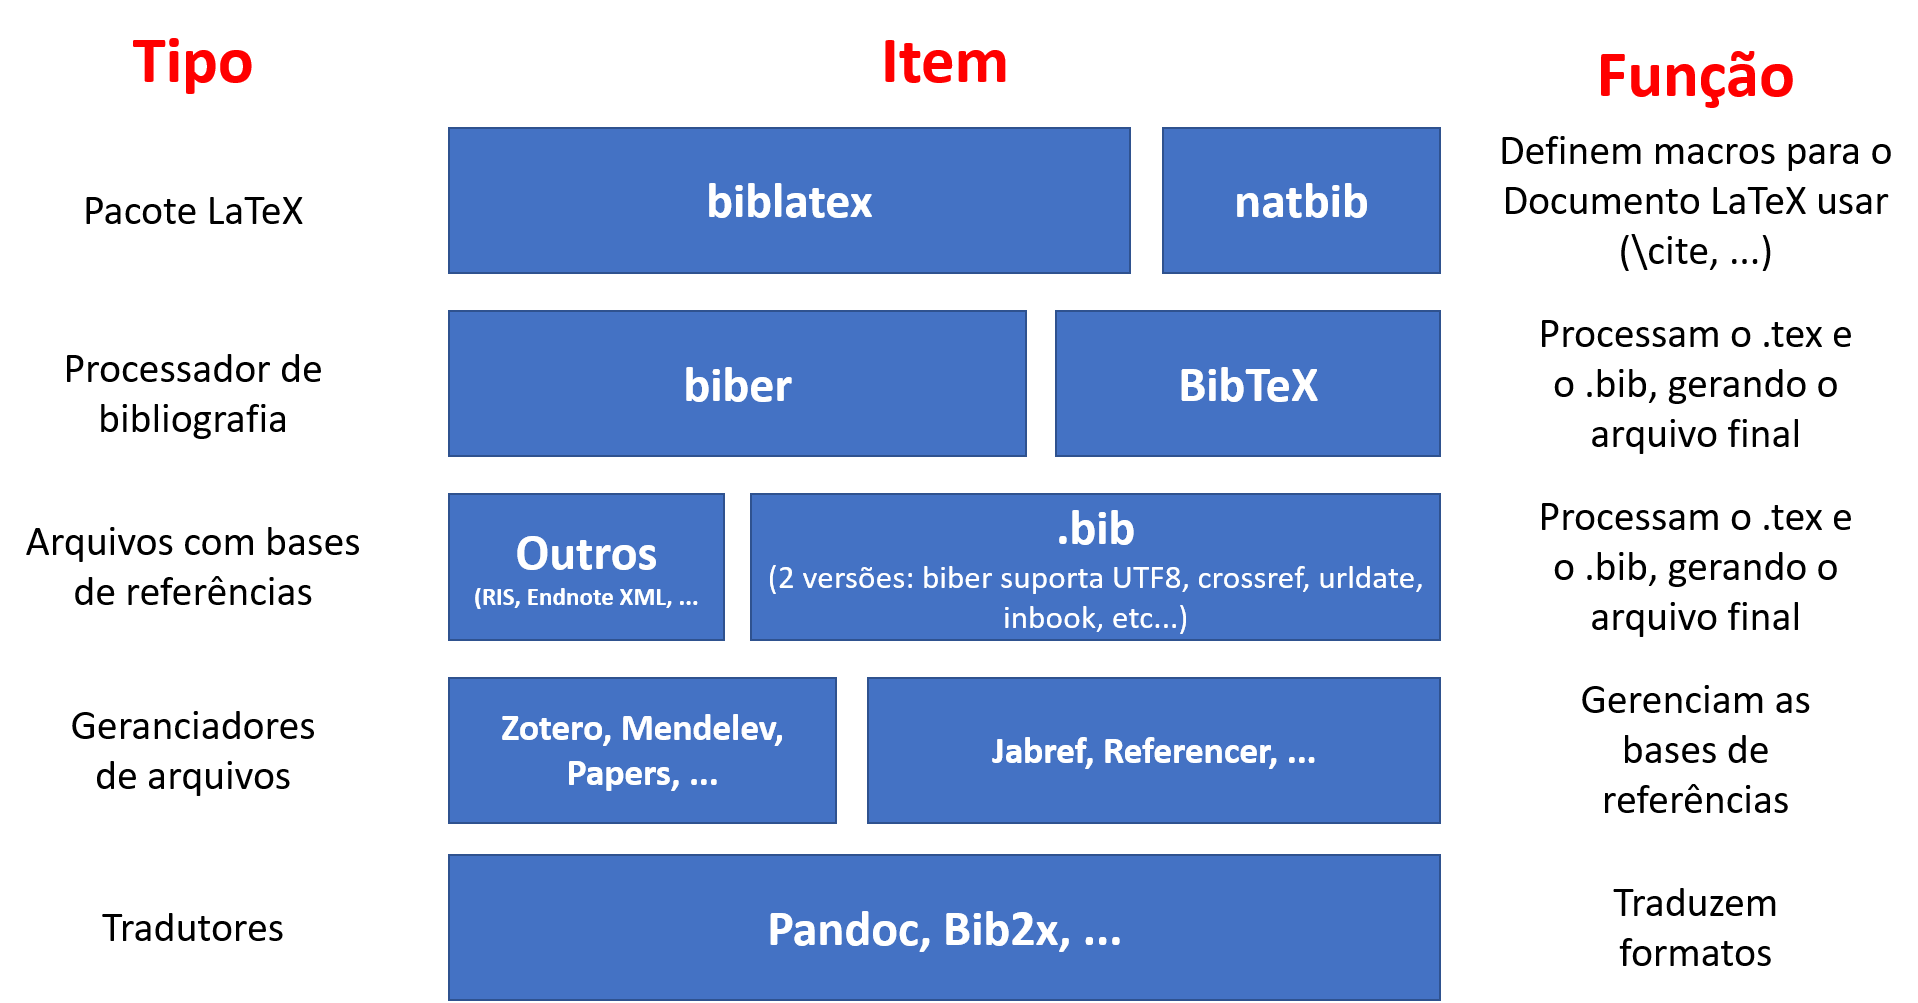
\includegraphics[width=0.9\linewidth]{Images/mundolatexport}
    \label{fig:mundolatexport}
\end{figure}
\end{frame}

\subsection{Como Funciona}
\begin{frame}{Como Funciona}
    \begin{figure}
        \centering
        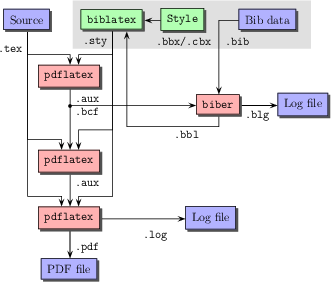
\includegraphics[width=0.7\linewidth]{Images/xMUL7}
        \caption{}
        \label{fig:xmul7}
    \end{figure}
    ..
\end{frame}

\subsection{natbib vs biblatex}
\begin{frame}[shrink=10]{natbib vs biblatex\autocite{biber:2012}}
    \begin{columns}
        \begin{column}{0.5\linewidth}
\begin{outline}
    \1 natbib
    \2 Antigo e estável, mantido mas não evoluído
    \2 Vantagens
    \3 Vários formatos já definidos (arquivos .bst)
    \3 Possui um pacote custom-bib, com o aplicativo makebst, que gera estilos bibliográficos, .bst, iterativamente
    \2 Desvantagens
    \3 Depende do \hologo{BibTeX} 
    \3 .bst é difícil de fazer (linguagem posfixa)
    \3 Orientado para autor-ano e numérico, mas não autor-título
\end{outline}
        \end{column}
    \begin{column}{0.5\linewidth}
\begin{outline}
    \1 biblatex
    \2 Ativamente desenvolvido
    \2 Ligado ao backend \hologo{biber}
    \2 Vantagens
    \3 Mais campos
    \3 Unicode no arquivo .bib
    \3 Usa métodos de \LaTeX\ para controle fino da sua bibliografia
    \2 Desvantagens
    \3 Algumas revistas podem não aceitar (porque não fizeram o \textit{upgrade} de seus estilos
\end{outline}
    \end{column}
    \end{columns}

\end{frame}

\subsection{\hologo{BibTeX} vs \hologo{biber}}
\begin{frame}[t]{\hologo{BibTeX} vs \hologo{biber}}
    \begin{columns}[t]
    \begin{column}{0.5\linewidth}
        \begin{outline}
            \1 \hologo{BibTeX}
            \2 Se for obrigado, use 
            \2 Estável e debugado
            \2 Problemas com caracteres não padrão como ä
        \end{outline}
    \end{column}
    \begin{column}{0.5\linewidth}
        \begin{outline}
            \1  \hologo{biber}
            \2 Prefira usar o  biber
            \2 UTF8!
            \2 .bib file muito mais verificado
            \3 Dá erros novos
            \2 Só funciona com biblatex
        \end{outline}
    \end{column}
\end{columns}
\end{frame}




\subsection{Programas Externos}
\begin{frame}{Programas Externos}
    \begin{outline}
        \1 JabRef (Java)
        \1 Referencer (GNOME)
        \1 Bib2x 
        \1 Zotero+Better BibTeX for Zotero
    \end{outline}
\end{frame}

\section{Usando biblatex e \hologo{biber}}
\begin{frame}[fragile]{Usando biblatex e \hologo{biber}}
    \begin{verbatim}
\usepackage{csquotes,xpatch}
\usepackage[backend=biber,style=numeric]{biblatex}
\addbibresource{references.bib}
...
\cite{biber:2012}
...
\printbibliography
    \end{verbatim}
\end{frame}


\subsection{Controlando a forma de citação}
\begin{frame}[fragile]{Controlando a forma de citação}
    \begin{verbatim}
    \usepackage{csquotes,xpatch}
    \usepackage[backend=biber,style=authordate,natbib]{biblatex}
    \addbibresource{references.bib}
    ...
    \citet{biber:2012}
    \citep{biber:2012}
    ...
    \printbibliography
    \end{verbatim}
\end{frame}


\begin{frame}[fragile]{Exemplo de citet e citep (natbib)}
    \begin{verbatim}
\documentclass{article}
\usepackage[T1]{fontenc}
\usepackage{csquotes,xpatch}
\usepackage[english,brazilian]{babel}
\usepackage[backend=biber,style=authoryear,natbib]{biblatex}
\addbibresource{references.bib}
\title{Meu Quinto Artigo}
\author{Geraldo Xexéo}
\begin{document}
\maketitle
\citet{biber:2012} não fala nada sobre isso. Mas \citep{biber1:2012} também não. Por isso \citep{biber:2012} não tem erro. 
\printbibliography       
\end{document}
    \end{verbatim}
\end{frame}

\begin{frame}{Como fica...}
% TODO: \usepackage{graphicx} required
\begin{figure}
    \centering
    \includegraphics[width=\linewidth]{quintoartigo.pdf}
\end{figure}
\end{frame}


\begin{frame}[fragile,shrink=20]{Exemplo dos comandos do biblatex}
    \begin{verbatim}
\documentclass{article}
\usepackage[T1]{fontenc}
\usepackage[english,brazilian]{babel}
\usepackage{csquotes,xpatch}
\usepackage[backend=biber,style=authoryear,natbib]{biblatex}
\addbibresource{references.bib}
\begin{document}
\autocite{biber:2012}

\cite{biber:2012}

\parencite{biber:2012}

\textcite{biber:2012}

Lorem\footcite{biber:2012}

\fullcite{biber:2012}

\printbibliography  
\end{document}
    \end{verbatim}
\end{frame}


\begin{frame}{Como fica...}
    \begin{figure}
        \centering
        \includegraphics[width=\linewidth]{sextoartigo.pdf}
    \end{figure}
\end{frame}

\section{.bib files}
\subsection{Conceituação básica dos .bib}
\begin{frame}{Conceituação básica dos .bib}
    \begin{outline}
        \1 Arquivos .bib
        \2 São bases de dados de registros bibliográficos
        \2 Formato totalmente legível
        \1 Entradas 
        \2 Cada entrada é de um tipo: book, article, ...
        \1 Campos
        \2 Campos obrigatórios para cada entrada
        \2 Campos opcionais
    \end{outline}
\end{frame}

\subsection{Exemplo de arquivo .bib}
\begin{frame}[fragile,shrink=20]{Exemplo de arquivo .bib}
    \begin{verbatim}
@book{sommerville:requirements,
author = {Sommerville, Ian and Sawyer, Pete},
title = {Requirements Engineering: A Good Practice Guide},
year = {1997},
isbn = {0471974447},
publisher = {John Wiley \& Sons, Inc.},
address = {USA},
edition = {1st}
}
@Article{therac25,
author       = {Nancy G. Levenson and Clark S. Turner},
title        = {An Investigation of the Therac-25 Accidentes},
journaltitle = {Computer},
date         = {1993-07},
volume       = {26},
number       = {7},
pages        = {18-41},
}
\end{verbatim}
\end{frame}

\subsection{Tipos de Entradas Mais Usados}
\begin{frame}{Tipos de Entradas Mais Usados}
\begin{itemize}
    \item article
    \item inbook
    \item book
    \item incollection
    \item collection
    \item inproceedings
    \item proceedings
    \item report
    \item thesis
    \item online
    \item misc
\end{itemize}
\end{frame}



\section{JabRef}
\subsection{JabRef}
\begin{frame}{JabRef}  
    \begin{figure}
        \centering
        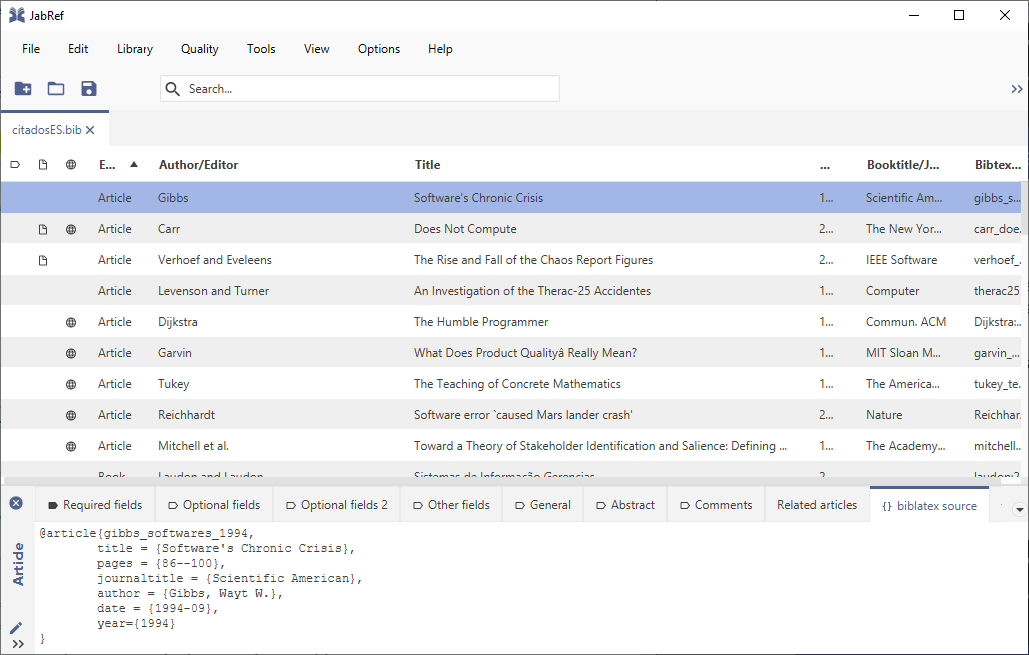
\includegraphics[width=0.7\linewidth]{Images/jabref}
    \end{figure}  
\end{frame}

\subsection{Características do JabRef}
\begin{frame}{Características do JabRef}
    \begin{itemize}
        \item Feito em Java
        \item Open Source
        \item Gerencia vários arquivos .bib em abas
        \item Permite unificar arquivos
        \item Suporte ao biblatex (UTF8,...)
        \item Detecta erros
        \item Busca na web
        \item ...
    \end{itemize}
\end{frame}

\section{Bibliografia}
\begin{frame}
        \printbibliography
\end{frame}


\begin{frame}
\Huge \center
Obrigado!
\end{frame} 

\begin{frame}{Contato}
\begin{center}
    
\includegraphics[width=\linewidth]{Images/Picture5.png}
\end{center}   
\end{frame}

\end{document}
